\chapter{Predictive Coding}

\acf{PC} is the theory that the ``purpose'' of the perceptual system is not to encode the maximum amount of information about the current state of the world, but rather to provide a prediction of the posterior distribution of the future state of the world. 

Indeed, this provides a parsimonious explanation for much of the brain's function. If you consider a video of two people talking in a living room with an old TV displaying static - most of the Shannon information in the video will be in the TV's display. While the speck of static may be a result of a particle left by the big bang hitting the antenna, our brain doesn't devote the majority of its resources to keep track of the white noise patterns. i.e. the brain's sensory processing system isn't designed to maximize the mutual information between the sensory signals it receives. Instead, if you consider the temporal information, the brain tries to encode the predictive information within its sensory streams. \PC has been hailed by some as ``The unifying theory of the brain.''

\PC provided the inspiration and fundamental theory behind temporal difference learning, a class of model free reinforcement learning methods which learn by bootstrapping from the current prediction of the state of the world. Temporal Difference Learning produced TD-Gammon which was beating humans even before the more famous Deep Blue eventually beat Kasparaov. Temporal Difference Learning is also one of inspirations for many of the current state-of-the-art reinforcement learning applications such as AlphaGo by DeepMind and Five by OpenAI.

If we were prescribed to the theory of \PC we would expect that somewhere the brain has to encode 1) the prediction of what is to come, and 2) the error between the prediction and what actually came to pass. Indeed, some of the most famous work in neuroscience has demonstrated these values in predictions of reward in dopamine signalling in the VTA. However, the theory of \PC would expect that these values should exist throughout the perceptual system as well for all aspects of the state of the world. A good place to look for this would be where the brain processes complex time-varying signals, namely, in auditory processing regions.

Surprise

``Indeed, a model-free approach seems out of the question in the context of video processing, as it would take unreasonably too many data samples and hence unreasonably too long to accumulate sufficient data and allow accurate model-free estimation of the underlying probability density function (PDF) of the data.''\cite{itti2005principled}

This is no longer true with modern machine learning techniques and methods for handling significantly more data than was possible in 2005. Therefore I have spent some effort building some models that predict future posterior probability density function of spectrograms.

\section{Models}

\subsection{Deep mixture of beta distributions}
My first attempt was to create a neural network that, given a window of spectrogram, predict the probability distribution of each frequency band in the next time bin of the spectrogram. The network was optimized by maximizing the log likelihood of the model. I modelled the probability distribution as a mixture of 3 beta distributions. The network was two fully connected layers with an output for a weight, $w$, and the two beta distribution parameters, $\alpha$ and $\beta$, for each of the three beta distributions, for each of the frequency bins. This network was very ill-behaved and I spent considerable time implementing as many numerical analysis tricks to control and regularize the networks exploding values. In the end I began to strip away as many of the complexities of the network as I could to create a minimum viable network.

\subsection{Deep Gaussian prediction}
This minimum network was to simply predict each frequency band as a univariate Gaussian with a mean and a standard deviation, and let the network try and deal with any covariances. This network trained easily enough, but didn't do nearly as good of a job at predicting as the deep mixture of beta distributions networks that were stopped before being corrupted by NaNs. However, even with this poor performance I did notice peaks in the likelihood that corresponded to motif boundaries.

\subsection{Contrastive Predictive Coding}
The last method I have explored is Contrastive Predictive Coding\cite{CPC}. CPC is a method that takes high dimensional time varying data, and attempts to do representation learning on it to provide a representation that captures the predictive information of the signal. They do this by encoding the high dimensional signal in a low dimensional latent space, $Z$, using an encoding network, and then feeding the latent space into a recurrent neural network which outputs a context in another latent space, $C$. $c_t$ is then used to linearly classify if a sample is actually the next time sample, or drawn from a distribution (I have used other random samples from the spectrogram). The whole model is learned end-to-end, providing an encoding information to a $Z$ space that both contains information that is useful for predictions, as well as information that is predictable. The model also provides the $C$ which also contains extra context from the past.

\begin{figure}[tbp] 
  \centering
  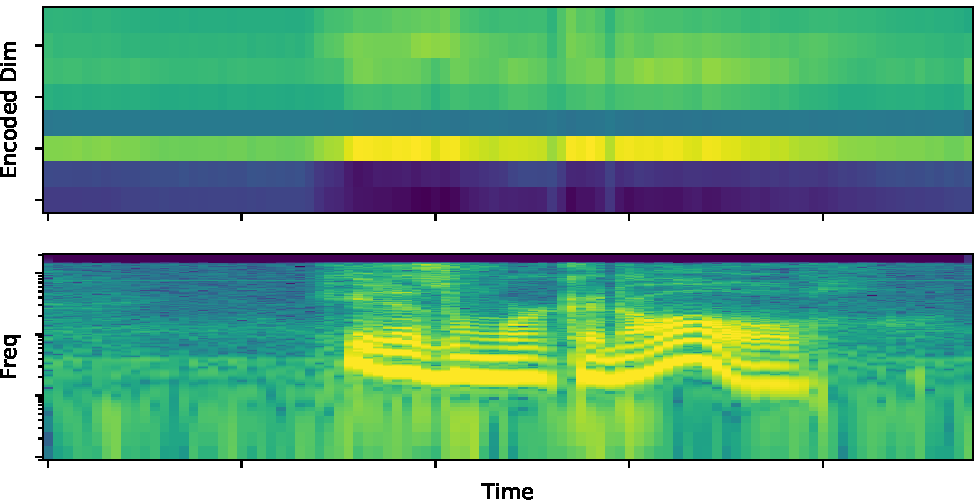
\includegraphics[width=\textwidth]{figures/encoder.pdf}
  \caption[8 dimensional $Z$ space learned by Contrastive Predictive Coding.]
{The representation learned by the encoder of CPC. Top: The 8 dimensional latent space $Z$ created by pushing each spectogram time slice through the encoder network. Bottom: 2048 Frequency bin spectrogram representation (not log spaced) fed into the encoder and the CPC network.
\index{encoder}}
  \label{fig:encoder}
\end{figure}

\subsection{Future Improvements}
 for CPC
wavenet style dilations
self attention
transformer networks
skip predictions

\section{Future Applications}

receptive field predictions

natural segmentation
